\documentclass[11pt]{article}
\usepackage[margin=1in]{geometry}
\usepackage{graphicx} 
\usepackage{amsmath}
\usepackage{bbm}
\usepackage{tikz}
\usepackage{titlesec}
\usepackage{hyperref}
\usepackage{booktabs}

\title{ACML Project 1 Report}

\author{
    Kent Liu \\
    \textit{Columbia University} \\
    \texttt{kjl2186@columbia.edu}
}

% Adjust section spacing
\titlespacing*{\section}{0pt}{*2}{*1.5}
\titlespacing*{\subsection}{0pt}{*1.5}{*1}

% Begin document
\begin{document}

\maketitle

\section*{Introduction}
With the recent advancement of technology in AI, we have access to more choices than ever when it comes to both hardware and models.  With this abundance, we are privileged to consider trade-offs based on performance, workload, and resource availability. In this report, I analyze the performance of select AI models across three different computing environments, providing insights into how hardware choices impact inference speed, computational efficiency, and overall feasibility. By analyzing the performance of select models across three different environments, we are able to gain some valuable insights about the choice of environment and models and potential tradeoffs for different workloads. The corresponding code can be found at \href{https://github.com/kentjliu/acml-project1}{This Github Link}.


\section*{Experiment Design}
With appropriate permissions and credits, Google Colab allows access to a variety of GPU runtimes. With this, we can compare different NN models from different domains and their performance in each environment. I will profile throughput and memory and use the roofline model to compare performance. In addition, I conduct some preliminary runs to gather data on compute utilization, memory bandwidth, and latency. By analyzing these factors, we can understand how different models behave under various hardware constraints and identify potential bottlenecks in system performance.

\section*{Complexity Estimation}
I expect more complex models (decreasing to increasing: ResNet, ViT, OPT) to require higher arithmetic intensity and memory movements and I expect more powerful GPUs (decreasing to increasing: T4, L4, A100) to perform better on greater workloads.
% I expect that model complexity will impact both arithmetic intensity and memory movement, with more complex models requiring higher computational resources. Specifically, I expect the complexity order to increase as follows: ResNet, ViT, OPT.

% Similarly, I expect more powerful GPUs to handle greater workloads more efficiently. In terms of performance capability, I expect the ranking to be: T4, L4, A100, with A100 delivering the highest performance.
% \section*{Measurement (Preliminary)}
\section*{Measurement}
In this section, we collect some preliminary roofline results, varying in batch size. We fix the model and environment.

\subsection*{Profiler Data}
Here, we collected some data from runs with the PyTorch profiler. We look at latency, throughput, GPU memory used, and CPU and CUDA times.

\subsubsection*{ResNet50}
\begin{table}[h]
    \centering
    \begin{tabular}{lccc}
        \toprule
        & T4 & L4 & A100 \\
        \midrule
        Avg Latency (ms) & 82.42 & 41.92 & 11.87 \\
        Throughput (images/s) & 388.24 & 763.35 & 2694.75 \\
        GPU Memory Used (MB) & 124.47 & 124.47 & 124.35 \\
        Self CPU time (ms) & 159.333 & 53.517 & 34.266 \\
        Self GPU time (ms) & 74.446 & 40.094 & 11.460 \\
        \bottomrule
    \end{tabular}
    \caption{ResNet performance with batch size 32. Latency decreases and throughput increases with increased GPU power. Memory usage is about the same due to fixed batch size.}
    \label{tab:gpu_comparison}
\end{table}

\subsubsection*{ViTb16}
\begin{table}[h]
    \centering
    \begin{tabular}{lccc}
        \toprule
        & T4 & L4 & A100 \\
        \midrule
        Avg Latency (ms) & 310.34 & 166.64 & 71.02 \\
        Throughput (images/s) & 103.11 & 192.03 & 450.59 \\
        GPU Memory Used (MB) & 356.85 & 356.85 & 356.85 \\
        Self CPU time (ms) & 329.951 & 166.828 & 88.754 \\
        Self GPU time (ms) & 319.239 & 154.940 & 70.991 \\
        \bottomrule
    \end{tabular}
    \caption{ViTb16 performance with batch size 32. Latency decreases and throughput increases with increased GPU power. Memory usage is about the same due to fixed batch size.}
    \label{tab:gpu_comparison}
\end{table}

\subsubsection*{OPT}

\begin{table}[h]
    \centering
    \begin{tabular}{lccc}
        \toprule
        & T4 & L4 & A100 \\
        \midrule
        Avg Latency (ms) & 63.11 & 57.36 & 23.12 \\
        Throughput (tokens/s) & 15.84 & 17.43 & 43.25 \\
        GPU Memory Used (MB) & 12708.16 & 12708.16 & 12708.16 \\
        Self CPU time (ms) & 86.820 & 79.407 & 120.470 \\
        Self GPU time (ms) & 59.276 & 54.937 & 13.388 \\
        \bottomrule
    \end{tabular}
    \caption{ViTb16 performance with the prompt "Columbia University is the best ". Latency decreases and throughput increases with increased GPU power. Memory usage is about the same due to fixed batch size.}
    \label{tab:gpu_comparison}
\end{table}


\section*{Isolated Roofline Runs}
\subsection*{ResNet50 (100 Runs)}
For ResNet, testing was done across various batch sizes: 1, 8, 16, 32, 64 to allow us to see effects of parallelism on compute and memory.
\subsubsection*{T4}
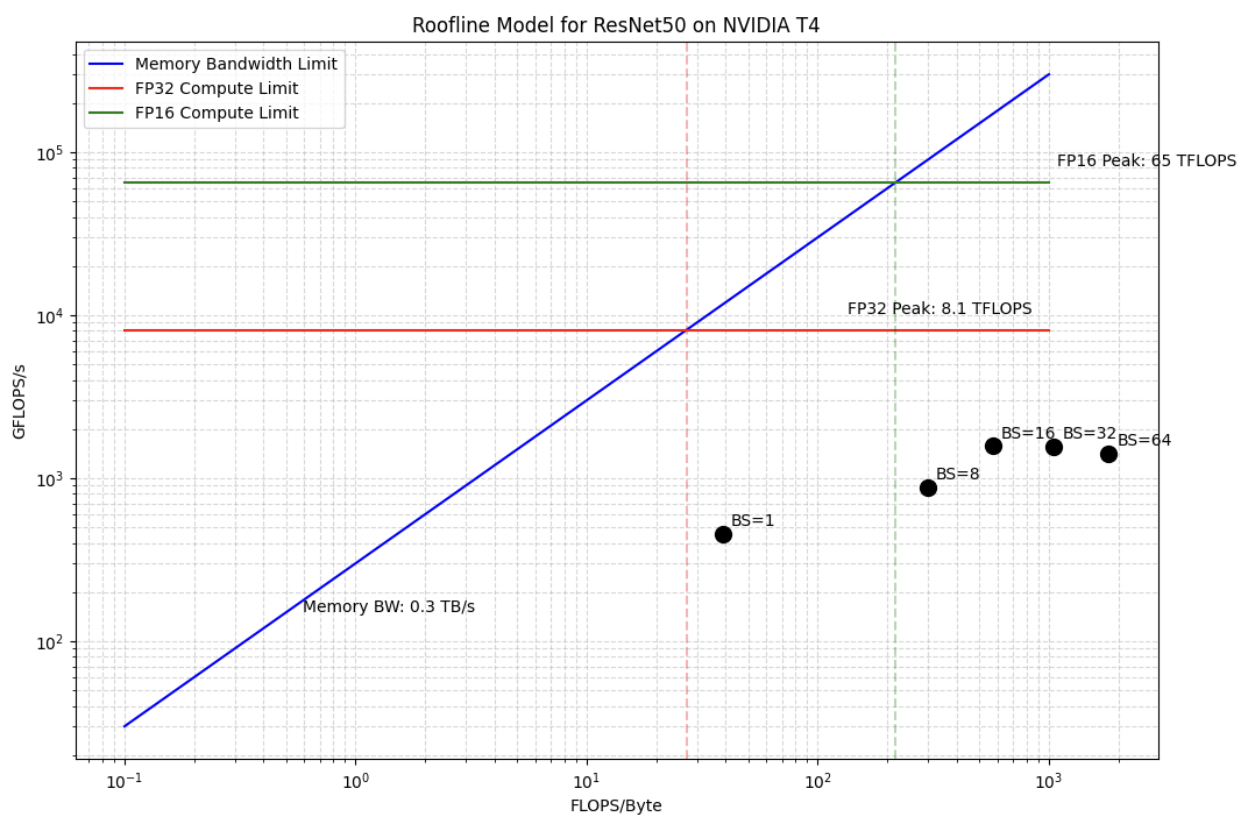
\includegraphics[width=14cm]{resnet/resnet_t4.png}
\subsubsection*{L4}
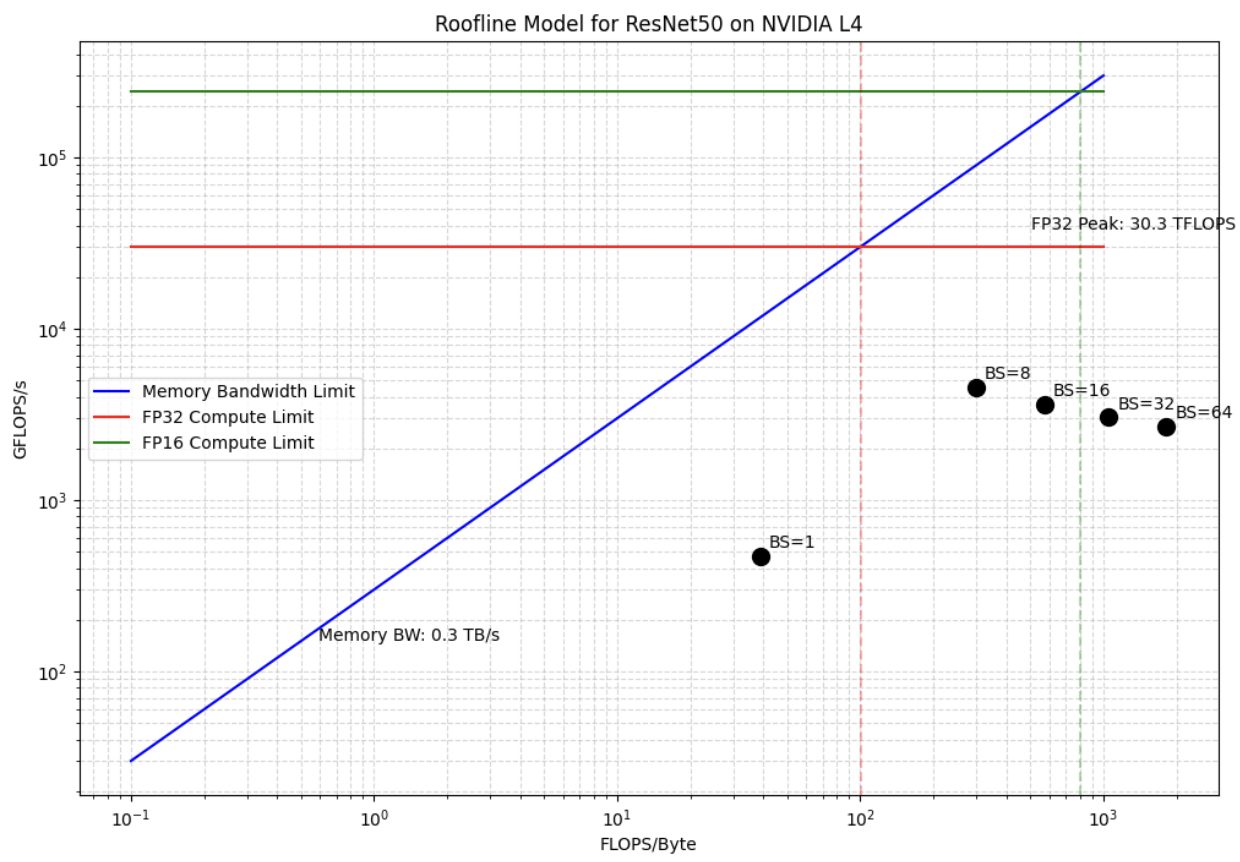
\includegraphics[width=14cm]{resnet/resnet_l4.png}
\subsubsection*{A100}
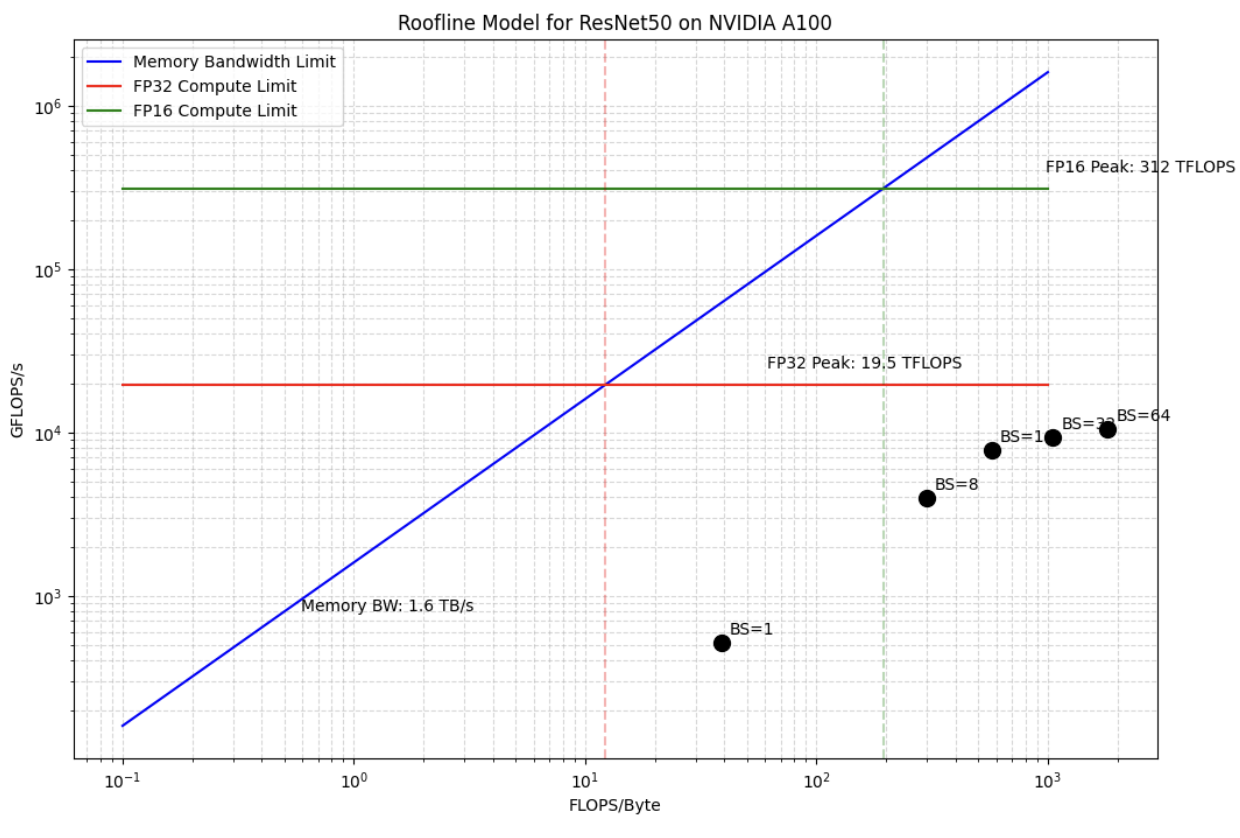
\includegraphics[width=14cm]{resnet/resnet_a100.png}


\subsection*{ViTb16 (100 Runs)}
Similar to ResNet, ViT testing was done across various batch sizes of 1, 8, 16, 32, 64 to allow us to see effects of parallelism on compute and memory.
\subsubsection*{T4}
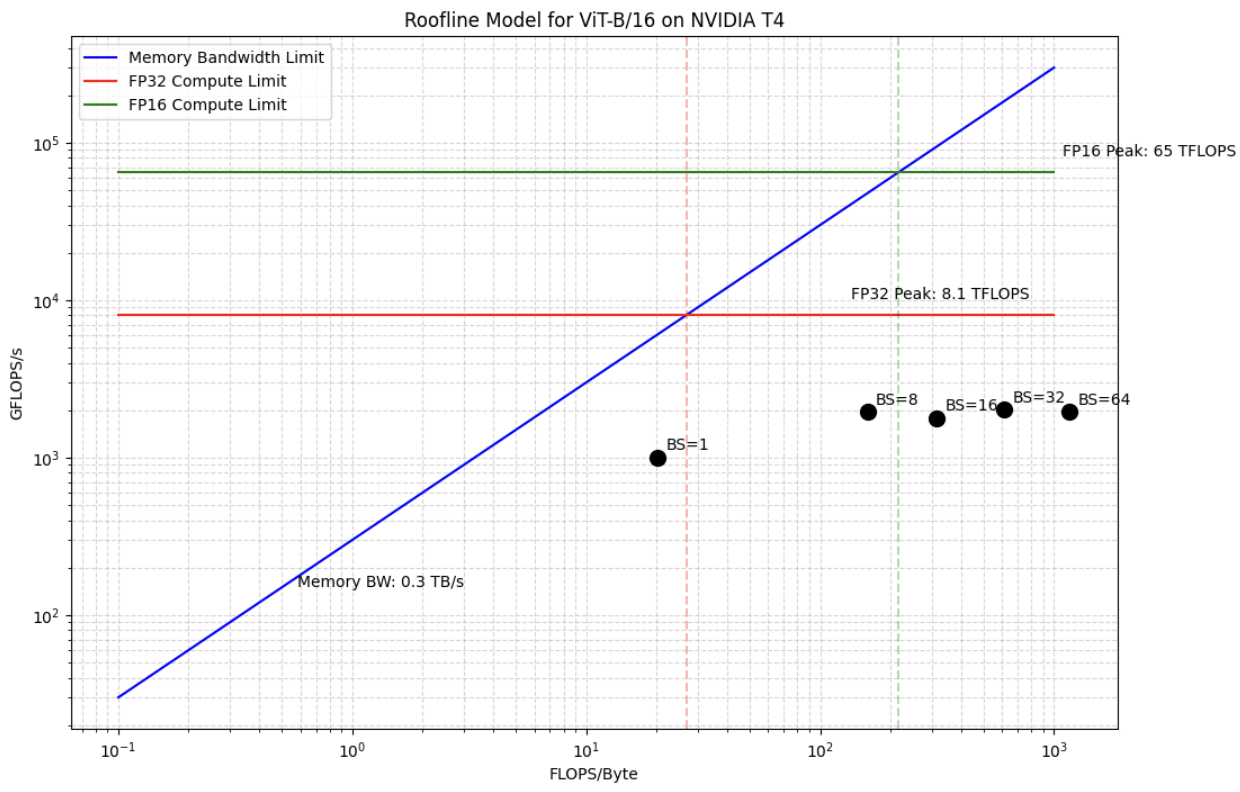
\includegraphics[width=14cm]{vit/vit_t4.png}
\subsubsection*{L4}
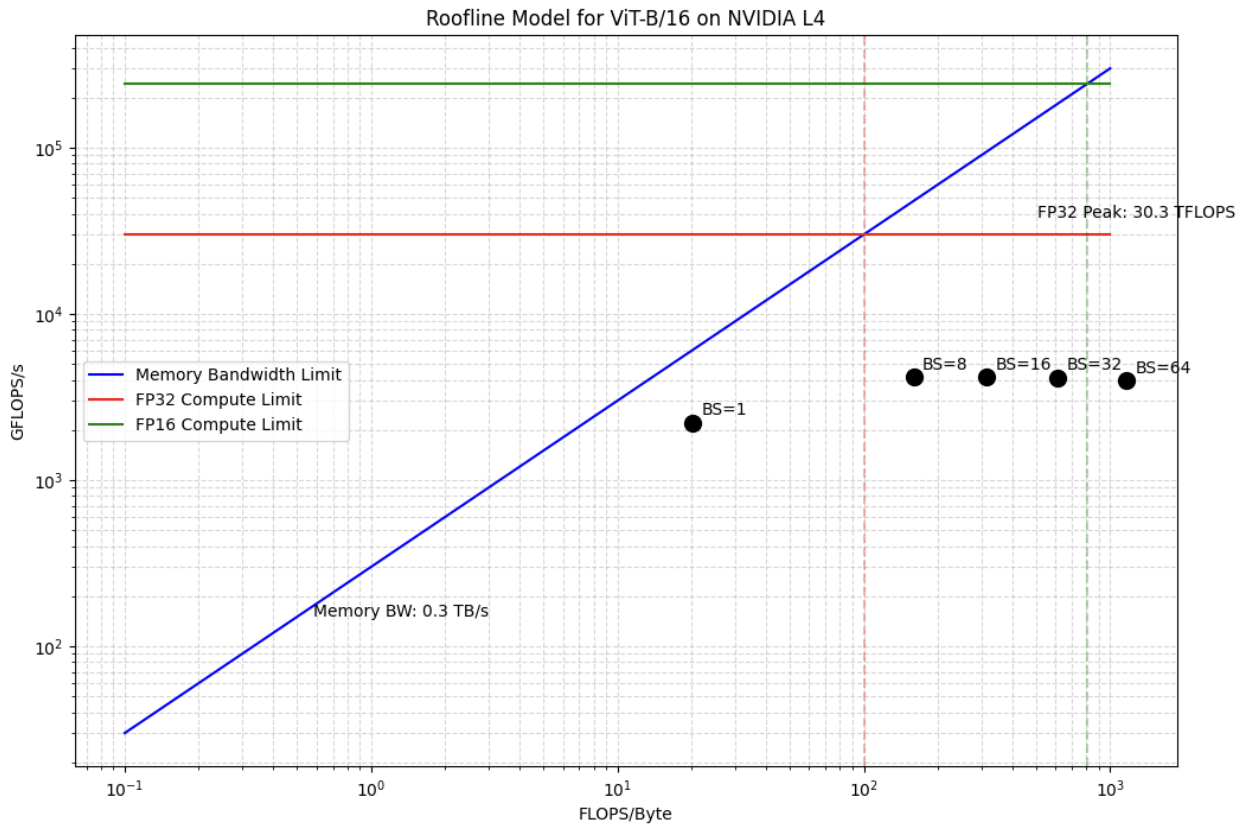
\includegraphics[width=14cm]{vit/vit_l4.png}
\subsubsection*{A100}
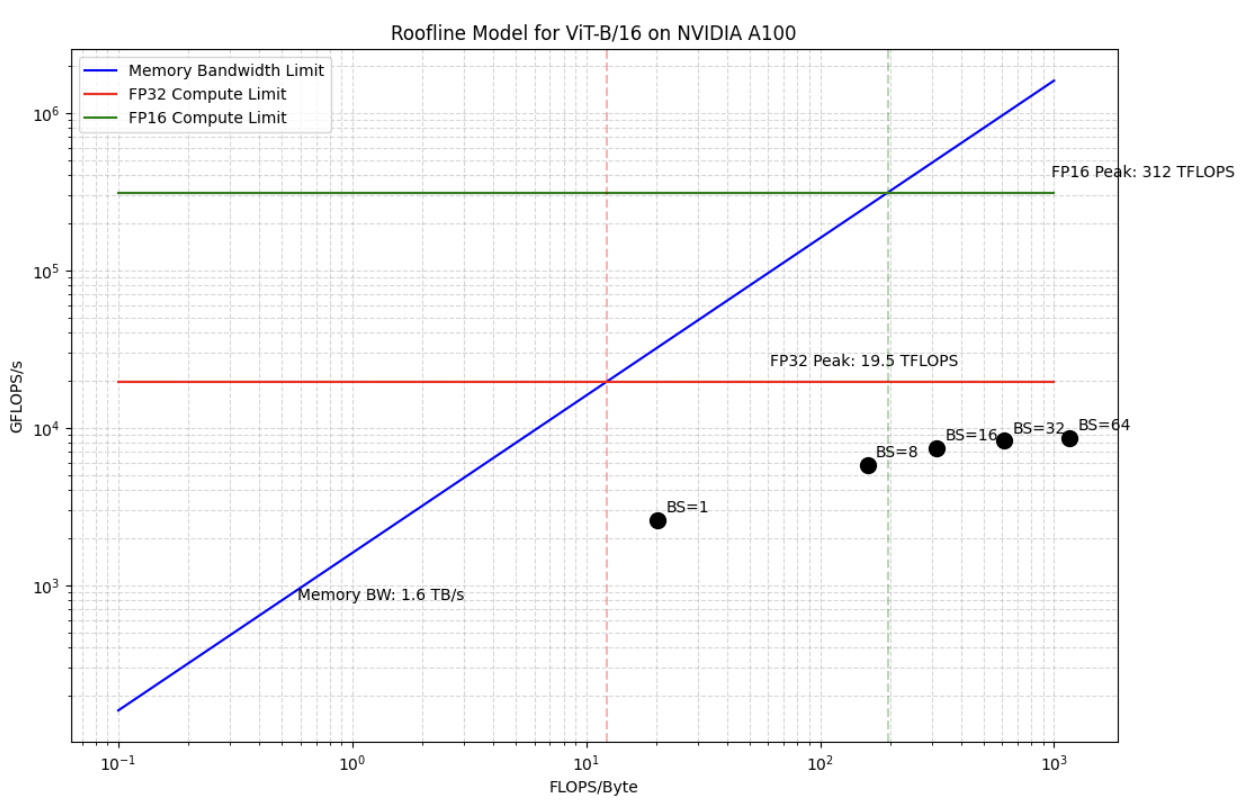
\includegraphics[width=14cm]{vit/vit_a100.png}

\subsection*{OPT-6.7b (100 Runs)}
Because Facebook's OPT model is a large language model, its inputs are processed in terms of tokens. By this token, we vary sequence lengths across runs: 35, 67, 131, 259, 515.
\subsubsection*{T4}
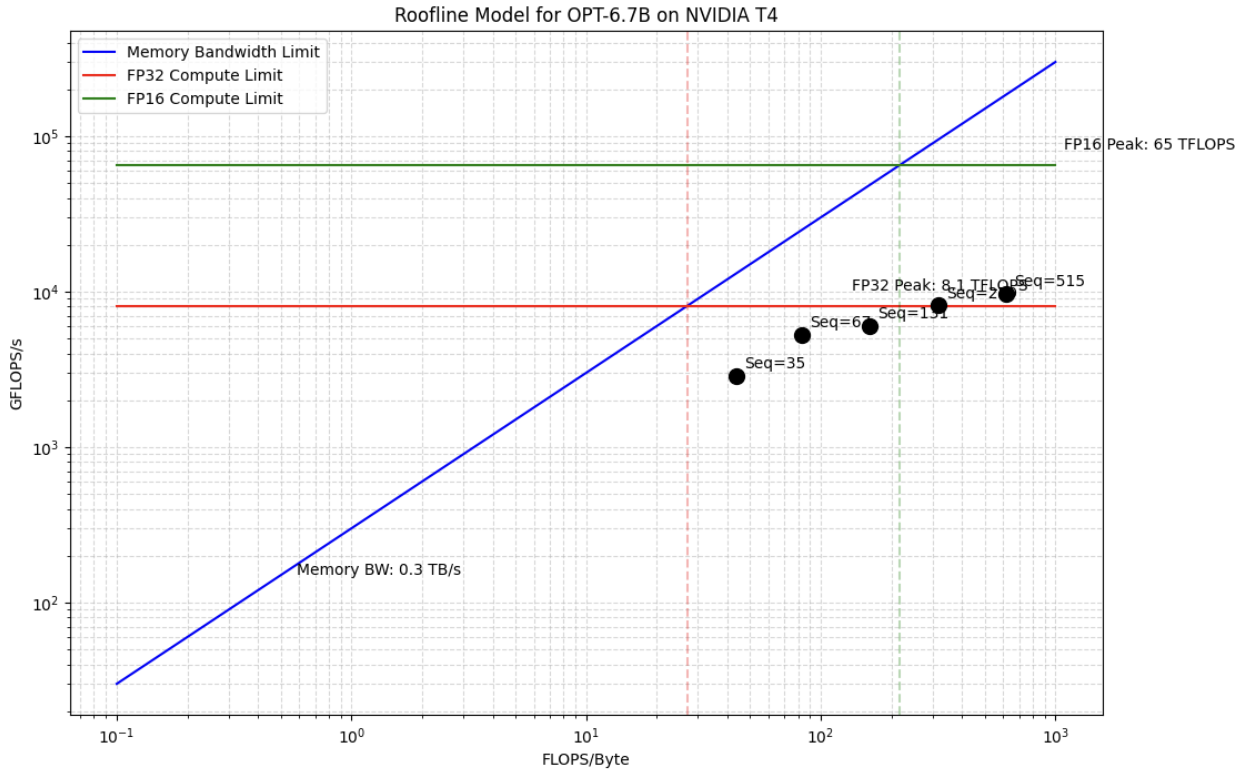
\includegraphics[width=14cm]{opt/opt_t4.png}
\subsubsection*{L4}
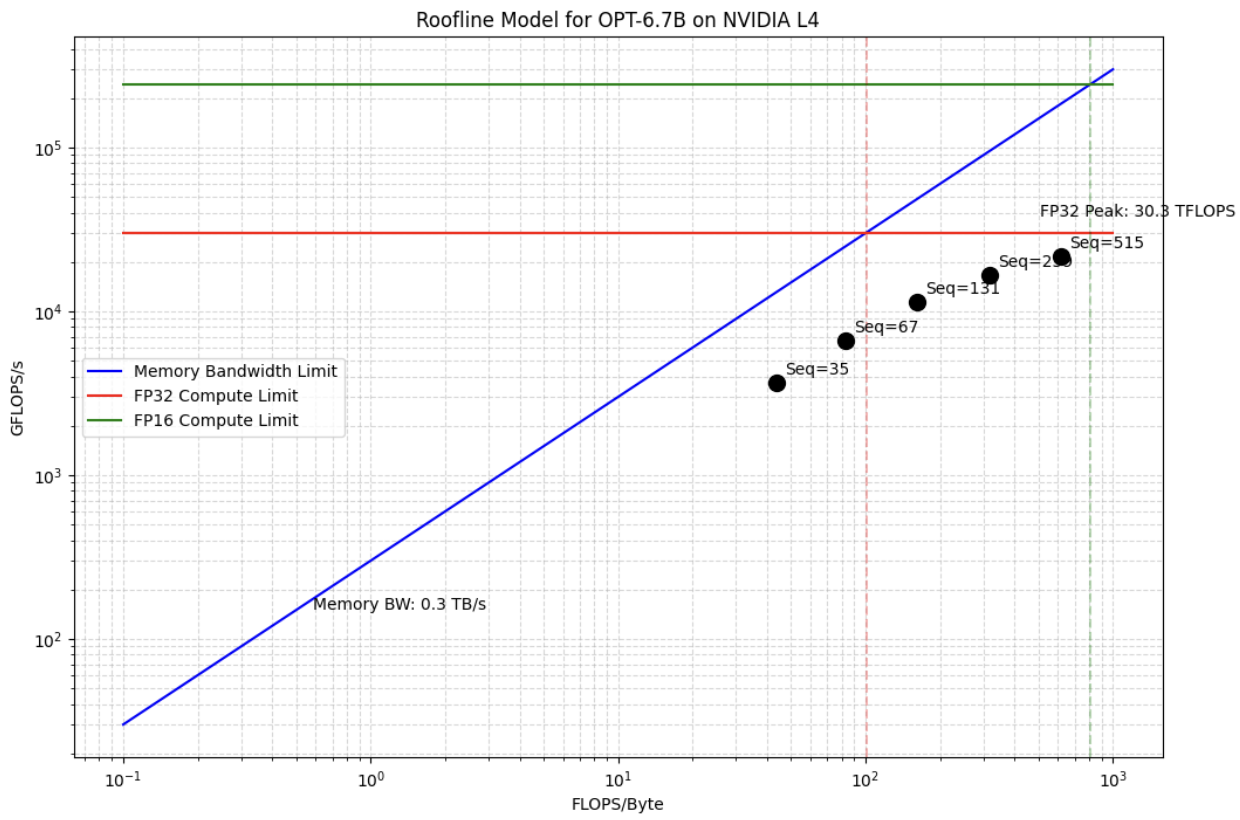
\includegraphics[width=14cm]{opt/opt_l4.png}
\subsubsection*{A100}
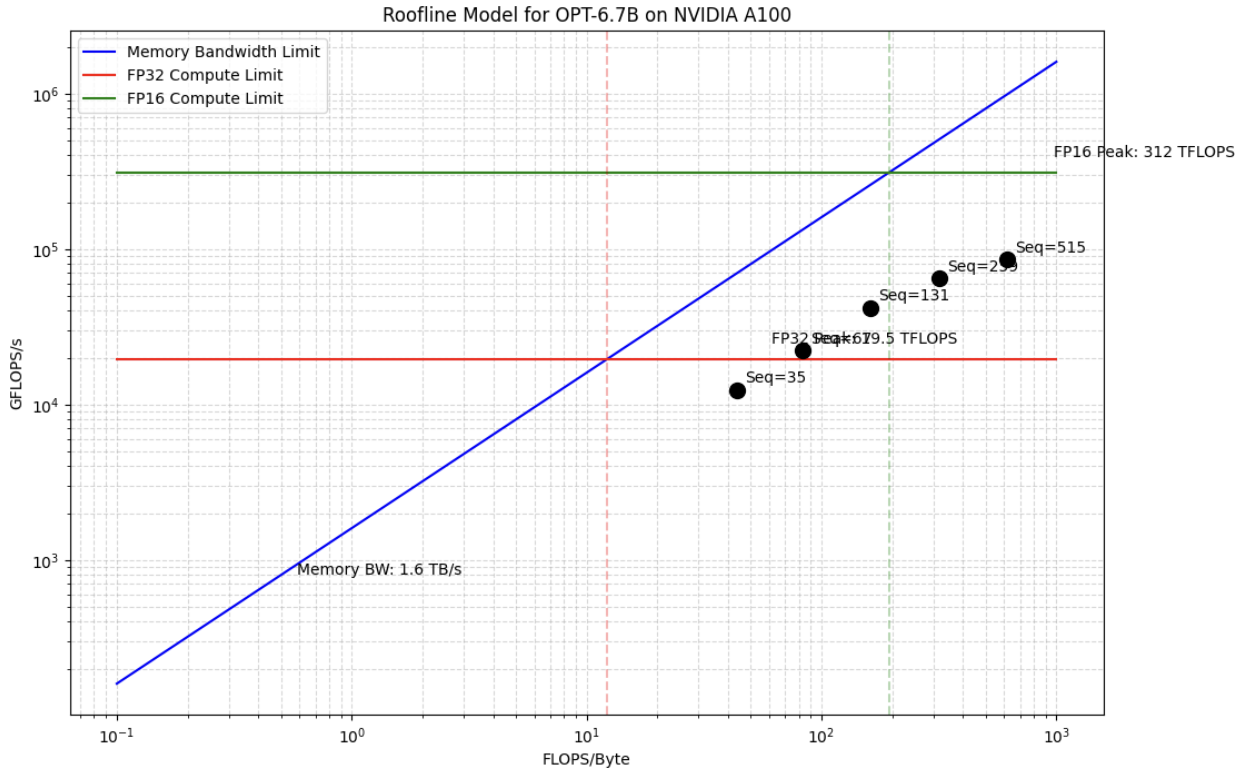
\includegraphics[width=14cm]{opt/opt_a100.png}


\section*{Roofline Modeling}
\subsubsection*{T4}
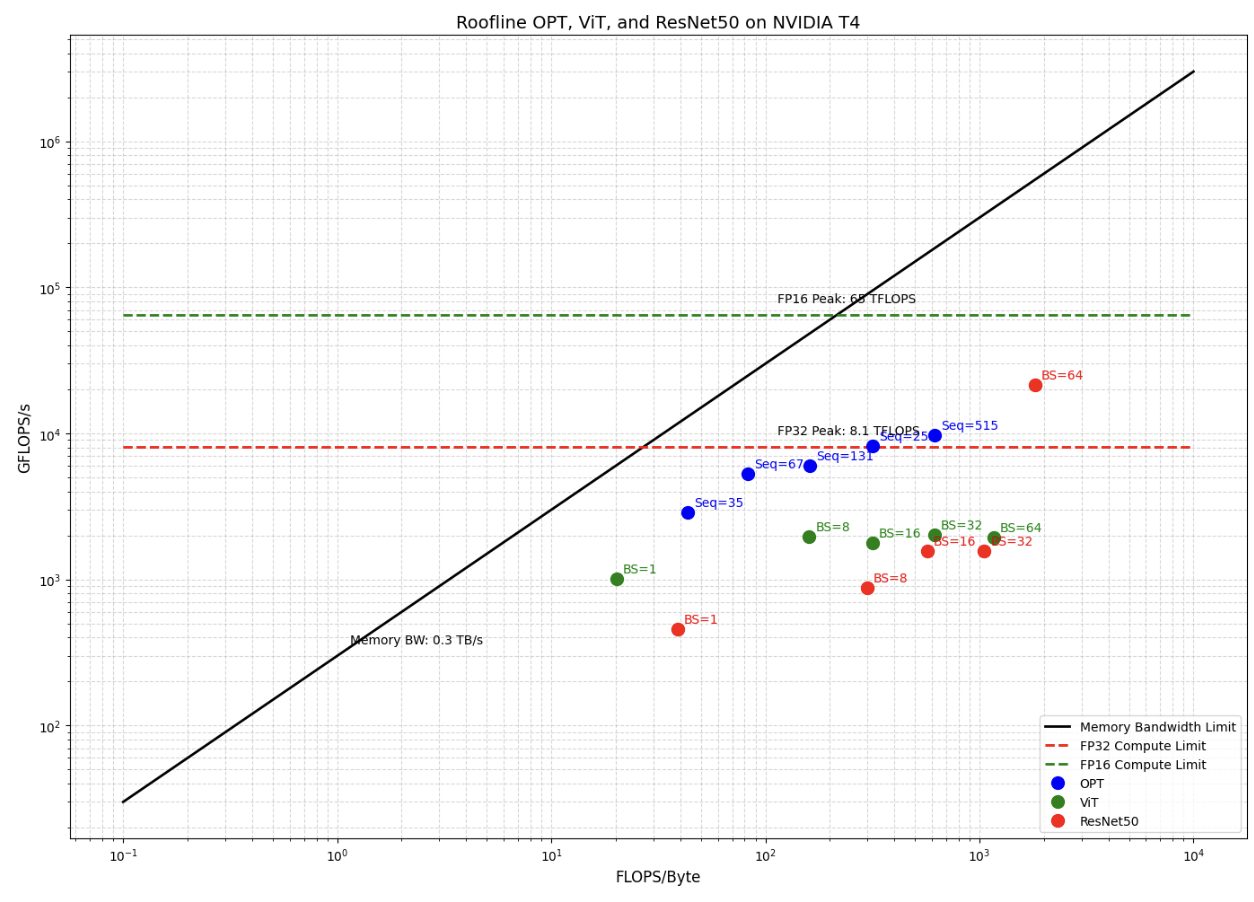
\includegraphics[width=14cm]{roofline/t4_roofline.png}
\subsubsection*{L4}
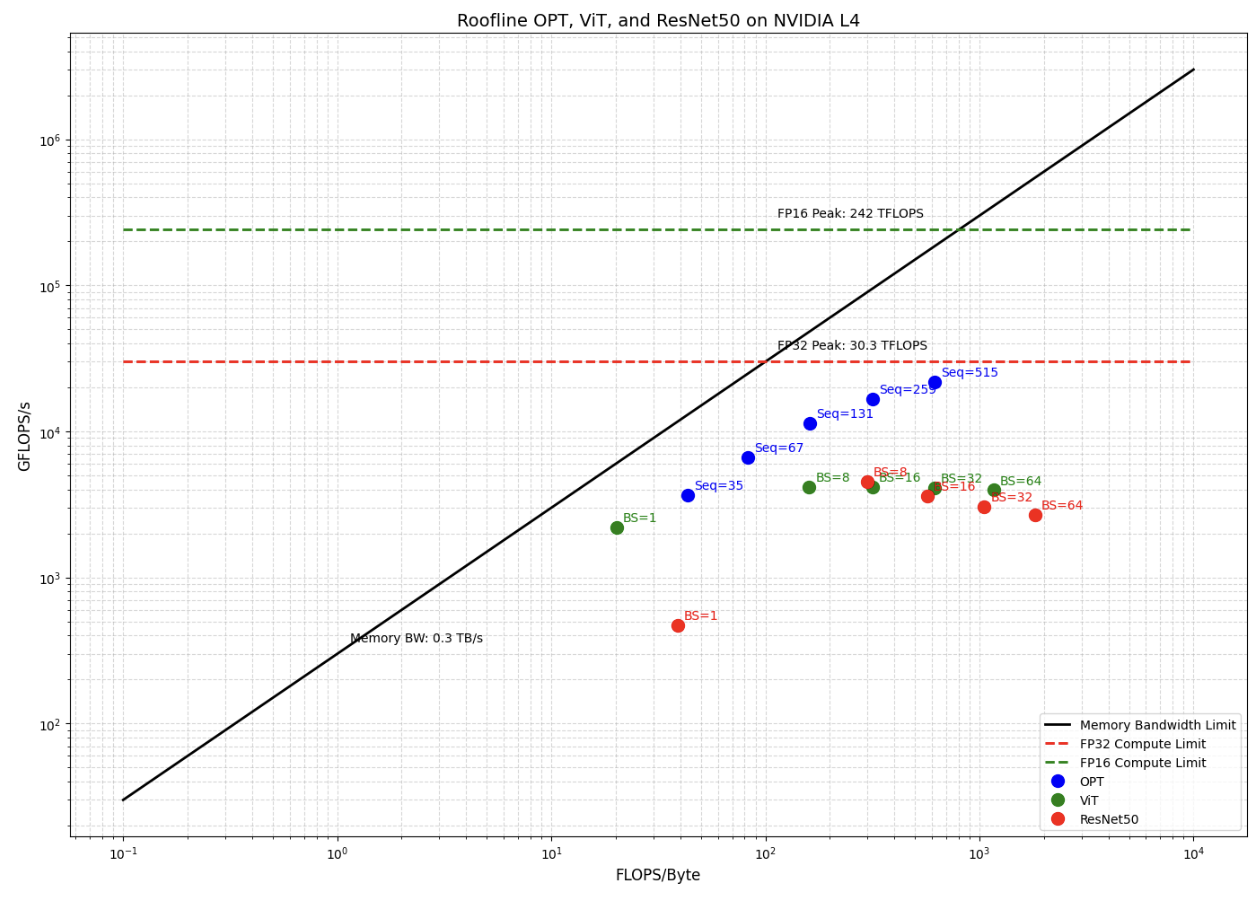
\includegraphics[width=14cm]{roofline/l4_roofline.png}
\subsubsection*{A100}
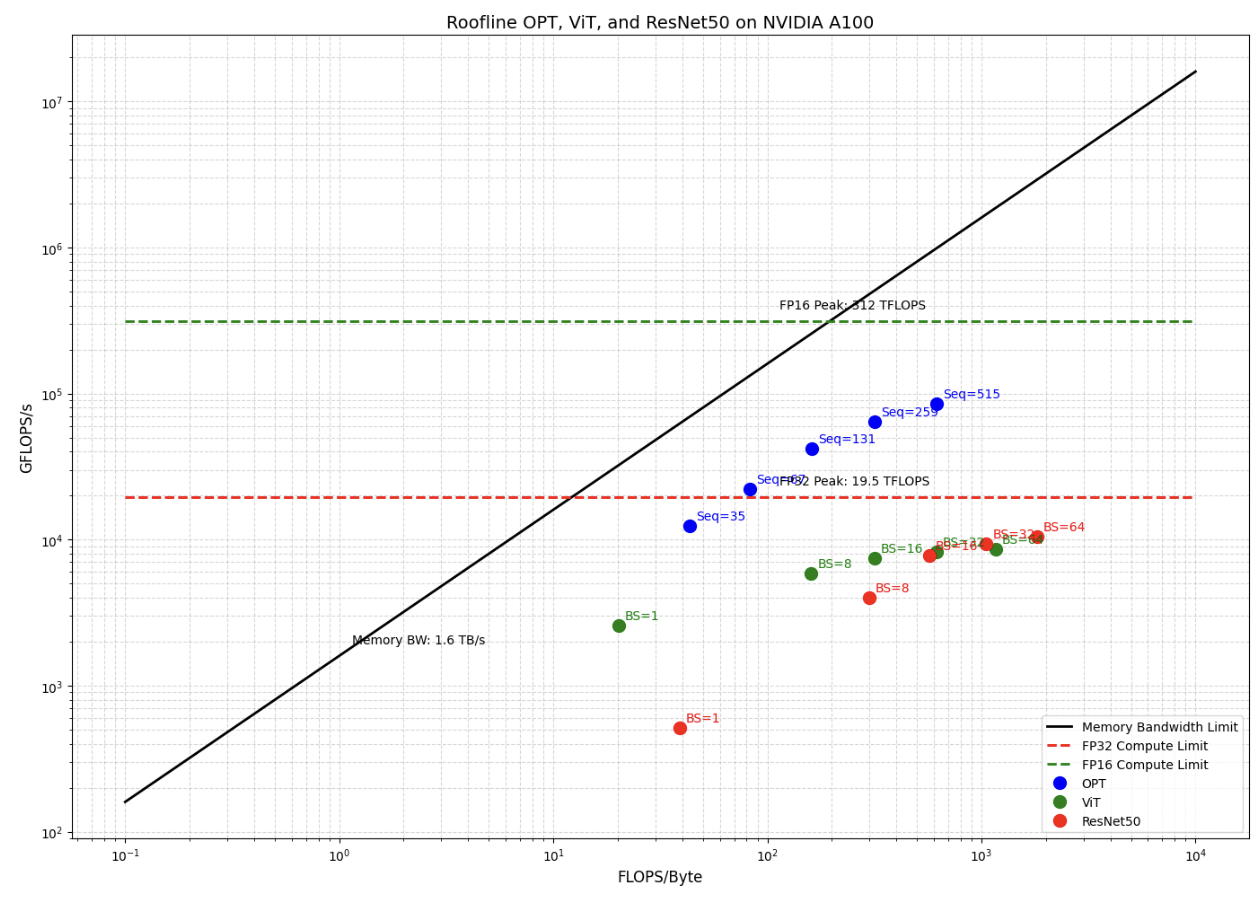
\includegraphics[width=14cm]{roofline/a100_roofline.png}

\section*{Analysis}
From the PyTorch profiler data, we see a decrease in latency and increase in throughput with higher performance environments, likely a testament to the increased power of the cores and better parallelism. In terms of latency across the models here, we observe that ResNet has the lowest latency, which makes sense as it is the least complex of the three models. However, we see that the ViT model having almost 6-8 times higher latency than OPT. However, we must remember that OPT processes items in terms of tokens as opposed to images, which are more complex in their data and structure.

As expected, from the previous three roofline graphs, even across varying batch sizes, the GFLOPS/s increased with the complexity of the model, with OPT requiring higher amounts. Additionally, as expected, higher batch sizes and sequence lengths increased the operational intensity. One thing to note is that all parameters in the OPT model are in FP16, explaining why some points exceed the FP32 threshold.

To be fair, the models were feasible enough to where they were not pushing the GPUs to the point of being memory and compute bound. For background, insight was gained from the datasheets of the respective GPUs, starting with the lowest compute and memory bandwidth T4 to the powerful and renowned A100. As batch size and sequence length increased, we were able to get more GFLOPS/s with stronger GPUs.

An interesting thing to note is that in some plots, there are sometimes decreases in GLOPS/s with increasing batch sizes. This might be due to memory bottlenecks or other resource limitations, like the GPU's internal bandwidth or cache management, where increasing the batch size too much starts to cause diminishing returns on throughput. This is a common phenomenon in deep learning workloads where performance doesn’t scale linearly with batch size after a certain point.

Overall, the results highlights the impact of model complexity and hardware capability on performance metrics such as latency, throughput, and GFLOPS/s. As expected, more powerful GPUs demonstrate improved efficiency, particularly for larger batch sizes and more computationally intensive models. However, we also observe that increasing batch size does not always lead to linear performance gains, likely due to memory bottlenecks and hardware constraints.


\bibliographystyle{plain}
\bibliography{references}
\subsection*{GPU Specifications from NVIDIA Datasheets (for Roofline Modeling)}
\begin{itemize}
    \item \textbf{A100}: \href{https://www.nvidia.com/content/dam/en-zz/Solutions/Data-Center/a100/pdf/nvidia-a100-datasheet.pdf}{NVIDIA A100 Datasheet}
    \item \textbf{L4}: \href{https://resources.nvidia.com/en-us-data-center-overview/l4-gpu-datasheet}{NVIDIA L4 Datasheet}
    \item \textbf{T4}: \href{https://www.nvidia.com/content/dam/en-zz/Solutions/Data-Center/tesla-t4/t4-tensor-core-datasheet-951643.pdf}{NVIDIA T4 Datasheet}
\end{itemize}

\subsection*{FLOPS Estimates for Selected Models}
\begin{itemize}
    \item \textbf{ResNet50 (224x224)}: Approx. 4 GFLOPS  
    \href{https://github.com/albanie/convnet-burden}{Source}
    \item \textbf{ViT-B/16}: Approx. 17.56 GFLOPS  
    \href{https://pytorch.org/vision/main/models/generated/torchvision.models.vit_b_16.html}{Source}
    \item \textbf{OPT Model}: FLOPS information available at  
    \href{https://huggingface.co/docs/transformers/en/model_doc/opt}{Hugging Face OPT Documentation}
\end{itemize}

\subsection*{Code} \textbf{Github}: 
    \href{https://github.com/kentjliu/acml-project1}{Repository Link}



\end{document}
